% Für Bindekorrektur als optionales Argument "BCORfaktormitmaßeinheit", dann
% sieht auch Option "twoside" vernünftig aus
% Näheres zu "scrartcl" bzw. "scrreprt" und "scrbook" siehe KOMA-Skript Doku
\documentclass[12pt,a4paper,titlepage,headinclude,bibtotoc]{scrartcl}


%---- Allgemeine Layout Einstellungen ------------------------------------------

% Für Kopf und Fußzeilen, siehe auch KOMA-Skript Doku
\usepackage[komastyle]{scrpage2}
\pagestyle{scrheadings}
\automark[section]{chapter}
\setheadsepline{0.5pt}[\color{black}]

%keine Einrückung
\parindent0pt

%Einstellungen für Figuren- und Tabellenbeschriftungen
\setkomafont{captionlabel}{\sffamily\bfseries}
\setcapindent{0em}

\usepackage{caption}

%---- Weitere Pakete -----------------------------------------------------------
% Die Pakete sind alle in der TeX Live Distribution enthalten. Wichtige Adressen
% www.ctan.org, www.dante.de

% Sprachunterstützung
\usepackage[ngerman]{babel}

% Benutzung von Umlauten direkt im Text
% entweder "latin1" oder "utf8"
\usepackage[utf8]{inputenc}

% Pakete mit Mathesymbolen und zur Beseitigung von Schwächen der Mathe-Umgebung
\usepackage{latexsym,exscale,amssymb,amsmath}

% Weitere Symbole
\usepackage[nointegrals]{wasysym}
\usepackage{eurosym}

% Anderes Literaturverzeichnisformat
%\usepackage[square,sort&compress]{natbib}

% Für Farbe
\usepackage{color}

% Zur Graphikausgabe
%Beipiel: \includegraphics[width=\textwidth]{grafik.png}
\usepackage{graphicx}

% Text umfließt Graphiken und Tabellen
% Beispiel:
% \begin{wrapfigure}[Zeilenanzahl]{"l" oder "r"}{breite}
%   \centering
%   \includegraphics[width=...]{grafik}
%   \caption{Beschriftung} 
%   \label{fig:grafik}
% \end{wrapfigure}
\usepackage{wrapfig}

% Mehrere Abbildungen nebeneinander
% Beispiel:
% \begin{figure}[htb]
%   \centering
%   \subfigure[Beschriftung 1\label{fig:label1}]
%   {\includegraphics[width=0.49\textwidth]{grafik1}}
%   \hfill
%   \subfigure[Beschriftung 2\label{fig:label2}]
%   {\includegraphics[width=0.49\textwidth]{grafik2}}
%   \caption{Beschriftung allgemein}
%   \label{fig:label-gesamt}
% \end{figure}
\usepackage{subfigure}
\usepackage{adjustbox}

% Caption neben Abbildung
% Beispiel:
% \sidecaptionvpos{figure}{"c" oder "t" oder "b"}
% \begin{SCfigure}[rel. Breite (normalerweise = 1)][hbt]
%   \centering
%   \includegraphics[width=0.5\textwidth]{grafik.png}
%   \caption{Beschreibung}
%   \label{fig:}
% \end{SCfigure}
\usepackage{sidecap}

% Befehl für "Entspricht"-Zeichen
\newcommand{\corresponds}{\ensuremath{\mathrel{\widehat{=}}}}

%Für chemische Formeln (von www.dante.de)
%% Anpassung an LaTeX(2e) von Bernd Raichle
\makeatletter
\DeclareRobustCommand{\chemical}[1]{%
  {\(\m@th
   \edef\resetfontdimens{\noexpand\)%
       \fontdimen16\textfont2=\the\fontdimen16\textfont2
       \fontdimen17\textfont2=\the\fontdimen17\textfont2\relax}%
   \fontdimen16\textfont2=2.7pt \fontdimen17\textfont2=2.7pt
   \mathrm{#1}%
   \resetfontdimens}}
\makeatother

%Si Einheiten
\usepackage{siunitx}

%c++ Code einbinden
\usepackage{listings}
\lstset{numbers=left, numberstyle=\tiny, numbersep=5pt}

%Differential
\newcommand{\dif}{\ensuremath{\mathrm{d}}}
%sinc
\newcommand{\sinc}{\ensuremath{\mathrm{sinc}}}

%Boxen,etc.
\usepackage{fancybox}
\usepackage{empheq}

%Fußnoten auf gleiche Seite
\interfootnotelinepenalty=1000

%Dateien aus Unterverzeichnissen
\usepackage{import}

%Bibliography \bibliography{literatur} und \cite{gerthsen}
%\usepackage{cite}
\usepackage{babelbib}
\selectbiblanguage{ngerman}

\begin{document}

\begin{titlepage}
\centering
\textsc{\Large Anfängerpraktikum der Fakultät für
  Physik,\\[1.5ex] Universität Göttingen}

\vspace*{4.2cm}

\rule{\textwidth}{1pt}\\[0.5cm]
{\huge \bfseries
  Beugung und Interferenz\\[1.5ex]
  von Laserlicht}\\[0.5cm]
\rule{\textwidth}{1pt}

\vspace*{3.0cm}

\begin{Large}
\begin{tabular}{ll}
Praktikant:
 	&  Felix Kurtz\\
 	&  Michael Lohmann\\

E-Mail: 
	&  felix.kurtz@stud.uni-goettingen.de\\
	& m.lohmann@stud.uni-goettingen.de\\

 Betreuer: & \\
 Versuchsdatum: &  09.03.2015\\
\end{tabular}
\end{Large}

\vspace*{0.8cm}

\begin{Large}
\fbox{
  \begin{minipage}[t][2.5cm][t]{6cm} 
    Testat:
  \end{minipage}
}
\end{Large}

\end{titlepage}

\tableofcontents

\newpage

\section{Einleitung}
\label{sec:einleitung}
In diesem Versuch sollen die Eigenschaften von Laserlicht für Beugung und Interferenz an verschiedenen Objekten genutzt werden.
Da ein Laser auf stimulierter Emission von Photonen basiert, ist sein Licht nämlich sehr monochromatisch sowie zeitlich und räumlich kohärent.
Als Lichtquelle wird diesmal ein Helium-Neon-Laser verwendet, der Intensitätsverlauf wird über eine mit einem Schrittmotor bewegbare Fotodiode elektronisch aufgenommen.

\section{Theorie}
\label{sec:theorie}
\subsection{Laserprinzip}
Wie der Name \textsc{Laser}, \textit{Light Amplification by Stimulated Emission of Radiation}, schon verrät, emittiert dieser Licht aufgrund Stimulierter Emission.
\begin{figure}[!h]
	\centering
	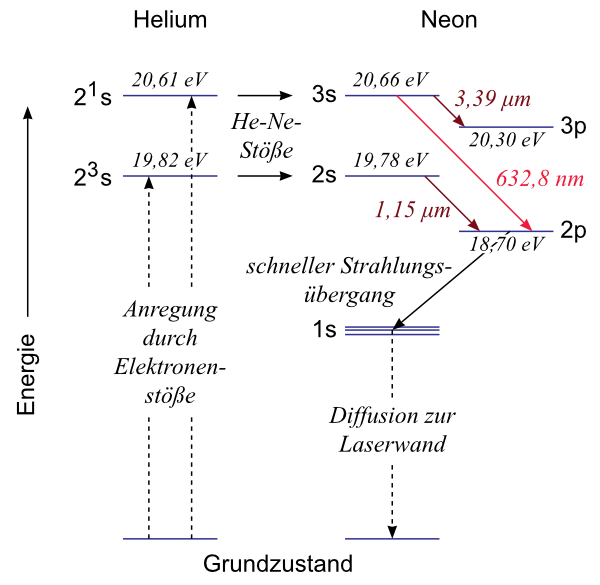
\includegraphics[scale=0.7]{NiveauHeNe.png}
	\caption{Niveauschema des Helium-Neon-Lasers. \cite[Datum: 02.01.15]{LP21}}
\end{figure}


\subsection{Beugung und Interferenz}
Das Fernfeld eines bestrahlten Objekts ergibt sich als Fouriertransformation des Feldes in der Objektebene.
Dies erhält man aus der Fraunhofer-Näherung des Fresnel-Kirchhoffschen Beugungsintegrals
\begin{align}
	E(x',y',z)=B(x,y)\cdot \int E(x,y,0)~ e^{-ik_xx} ~ e^{-ik_yy} ~\dif x~ \dif y \,.
	\label{eq:Fraunhofer}
\end{align}

\subsubsection{Doppelspalt}
Für einen Doppelspalt mit einem Spaltabstand $d$ und infinitesimaler Spaltbreite ergibt sich nach \eqref{eq:Fraunhofer} dieser Intensitätsverlauf
\begin{align}
	I(\varepsilon)=I_0 \cdot \cos^2(\varepsilon) \,.
\end{align}
Dabei ist $\varepsilon= \frac{\pi d \sin \alpha}{\lambda}$.

\subsubsection{Einzelspalt und Steg}
\begin{align}
	I(\varepsilon)=I_0 \cdot \sinc^2(\varepsilon)
\end{align}

\subsubsection{Kreisblende}
\begin{align}
	I(\varepsilon)=I_0 \cdot \left(\frac{J_1(\varepsilon)}{\varepsilon}\right)^2
\end{align}

\subsubsection{Mehrfachspalt}
\begin{align}
	I(\varepsilon)=I_0 \cdot \sinc^2\left(\frac{\pi\alpha D}{\lambda}\right) \cdot \left(\frac{\sin(N\varepsilon)}{\sin(\varepsilon)}\right)^2
\end{align}

\section{Durchführung}
\label{sec:durchfuehrung}
\begin{figure}[!h]
	\centering
	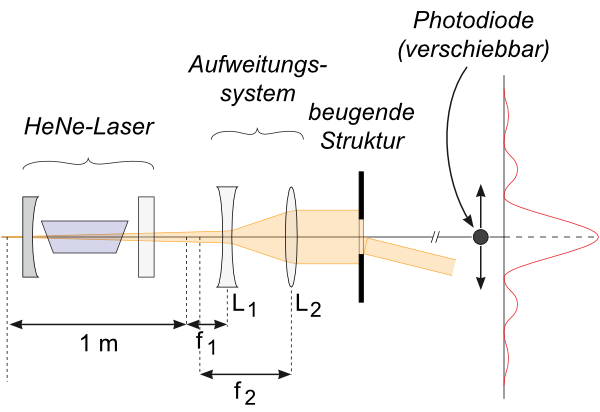
\includegraphics[scale=0.7]{Aufbau.png}
	\caption{Aufbau. \cite[Datum: 02.01.15]{LP21}}
\end{figure}

\section{Auswertung}
\label{sec:auswertung}

\section{Diskussion}
\label{sec:diskussion}

\section{Anhang}

\bibliography{literatur}
\bibliographystyle{babalpha}

\end{document}
